%        File: pres.tex
%     Created: Tues June 19 07:00 AM 2012 C
%
%\documentclass[11pt,handout]{beamer}
\documentclass[9pt]{beamer}

\usepackage{graphicx}
\usepackage{booktabs} % nice rules for tables
\usepackage{microtype} % if using PDF
\usepackage{bigints}
\newcommand{\units}[1] {\:\text{#1}}%
\newcommand{\SN}{S$_N$}%{S$_\text{N}$}%{$S_N$}%
\DeclareMathOperator{\erf}{erf}


\usetheme[white]{Wisconsin}
%\title[short title]{long title}
\title[Numerical Calibrations]{Numerical Calibrations of an Analytical Generic 
Nuclear Repository Heat Transfer Model} 
%\subtitle[short subtitle]{long subtitle}
\subtitle[ANS 2012]{American Nuclear Society Summer Meeting 2012} 
%\author[short name]{long name}
\author[Kathryn Huff]{Kathryn D.~Huff$^{1,2}$ \& Theodore H. Bauer$^2$}
%\date[short date]{long date}
\date[06.27.2012]{June 27, 2012}
%\institution[short name]{long name}
\institute[UW-Madison]{$^1$University of Wisconsin-Madison \& $^2$Argonne National Laboratory}
%Those icons in the references are terrible looking
\setbeamertemplate{bibliography item}[text]


\begin{document}
%%%%%%%%%%%%%%%%%%%%%%%%%%%%%%%%%%%%%%%%%%%%%%%%%%%%%%%%%%%%%
%% From uw-beamer Here's a handy bit of code to place at 
%% the beginning of your presentation (after \begin{document}):
\newcommand*{\alphabet}{ABCDEFGHIJKLMNOPQRSTUVWXYZabcdefghijklmnopqrstuvwxyz}
\newlength{\highlightheight}
\newlength{\highlightdepth}
\newlength{\highlightmargin}
\setlength{\highlightmargin}{2pt}
\settoheight{\highlightheight}{\alphabet}
\settodepth{\highlightdepth}{\alphabet}
\addtolength{\highlightheight}{\highlightmargin}
\addtolength{\highlightdepth}{\highlightmargin}
\addtolength{\highlightheight}{\highlightdepth}
\newcommand*{\Highlight}{\rlap{\textcolor{HighlightBackground}{\rule[-\highlightdepth]{\linewidth}{\highlightheight}}}}
%%%%%%%%%%%%%%%%%%%%%%%%%%%%%%%%%%%%%%%%%%%%%%%%%%%%%%%%%%%%%
%%--------------------------------%%
\frame{
\titlepage
}
%%--------------------------------%%
\AtBeginSection[]{
\begin{frame}[c!]
  \frametitle{Outline}
  \tableofcontents[currentsection]
\end{frame}
}

%%--------------------------------%%
%%--------------------------------%%

%        File: thermal.tex
%     Created: Mon June 19 07:00 AM 2012 C


\section{Motivation}
\subsection{Future Disposal System Options}
% Waste is a problem
% Decisionmakers are contemplating many fuel cycle options
% Decisionmakers are contemplating many repository options
% Interfacing between FCO/SA campaign and UFD campaign

\begin{frame}[ctb!]
  \frametitle{Future Disposal System Options}
   \begin{minipage}{0.44\textwidth}
     \begin{figure}[h!]
         \includegraphics[width=0.8\textwidth]{saltNewScientist.eps}
         \caption{U.S. Salt Deposits, ref. \cite{newscientist_where_2011}.}
     \end{figure}
     \begin{figure}[h!]
         \includegraphics[width=0.8\textwidth]{clayGonzales.eps}
         \caption{U.S. Clay Deposits, ref. \cite{gonzales_shales_1985}.}
     \end{figure}
   \end{minipage}
   \hspace{0.01cm}
   \begin{minipage}{0.44\textwidth}
     \begin{figure}[h!]
         \includegraphics[width=0.8\textwidth]{boreholeNewScientist.eps}
         \caption{U.S. Crystalline Basement, ref.  \cite{newscientist_where_2011}.}
     \end{figure}
     \begin{figure}[h!]
         \includegraphics[width=0.8\textwidth]{graniteBush.eps}
         \caption{U.S. Granite Beds, ref. \cite{bush_economic_1976}.}
     \end{figure}
   \end{minipage}
\end{frame}


\begin{frame}[ctb!]
  \frametitle{Future Fuel Cycle Options}
   % Future Fuel Cycles
    \begin{table}
      \centering
      \footnotesize{
      \begin{tabular}{|l|l|l|}
        \multicolumn{3}{c}{\textbf{Domestic Fuel Cycle Options}}\\
        \hline
        Title & Description& Challenges \\
        \hline
        \hline
        Open          & Once Through         & High Temperatures, Volumes \\
                      & Current US PWR Fleet &      \\
                      & No Separations       &      \\
                      & No Recycling         &      \\
                      & Higher Burnups &      \\
        \hline
        Modified Open & Partial Recycling    & Both high volumes and myriad fuel streams \\
                      & Next Gen. PWR Fleet &      \\
                      & Limited Separations  &      \\
                      & Limited Transmutation &      \\
                      & Advanced Fuel Forms  &      \\
                      & HLW treatment    &          \\
        \hline
        Closed        & Full Recycling       & Myriad fuel streams \\
                      & Full Separations &      \\
                      & Full Recycling &      \\
                      & VHTGR, SFRs, &      \\
                      & other transmutation & \\
                      & HLW treatment  &      \\
        \hline
      \end{tabular}
      \caption[Fuel Cycle Options]{Domestic Fuel Cycle Options }
      \label{tab:fco}
      }
    \end{table}
\end{frame}


% layouts
% EBS choices
% Geologies


\begin{frame}[ctb!]
  \frametitle{Clay Disposal Environments}

  \begin{figure}[h!]
    \begin{center}
      \includegraphics[height=.7\textheight]{belgianClayRedImp.eps}
    \end{center}
    \caption{Belgian reference concept in Boom Clay 
    \cite{von_lensa_red-impact_2008}.}
    \label{fig:belgianClayRedImp}
  \end{figure}

\end{frame}

\begin{frame}[ctb!]
  \frametitle{Granite Disposal Environments}

  \begin{figure}[h!]
    \begin{center}
      \includegraphics[height=.7\textheight]{czechGraniteRedImp.eps}
    \end{center}
    \caption{Czech reference concept in Granite 
    \cite{von_lensa_red-impact_2008}.}
    \label{fig:czechGraniteRedImp}
  \end{figure}

\end{frame}

\begin{frame}[ctb!]
  \frametitle{Salt Disposal Environments}

  \begin{figure}[h!]
    \begin{center}
      \includegraphics[height=.7\textheight]{saltGPAM.eps}
    \end{center}
    \caption{DOE-NE Used Fuel Disposition Campaign  concept in 
    Salt \cite{clayton_generic_2011}.}
    \label{fig:saltGPAM}
  \end{figure}

\end{frame}

\begin{frame}[ctb!]
  \frametitle{Deep Borehole Disposal Environment}

  \begin{figure}[h!]
    \begin{center}
      \includegraphics[height=.7\textheight]{boreholeGPAM.eps}
    \end{center}
    \caption{DOE-NE Used Fuel Disposition Campaign Deep Borehole concept 
    \cite{clayton_generic_2011}.}
    \label{fig:boreholeGPAM}
  \end{figure}

\end{frame}


\begin{frame}
  \frametitle{Repository Layouts}

  \begin{minipage}{0.49\textwidth}
    \begin{figure}[h!]
      \includegraphics[width=0.75\textwidth]{boreholes.eps}
    \end{figure}
    \begin{figure}[h!]
      \includegraphics[width=0.75\textwidth]{vertical.eps}
    \end{figure}
  \end{minipage}
  \hspace{0.01cm}
  \begin{minipage}{0.49\textwidth}
    \begin{figure}[h!]
      \includegraphics[width=0.8\textwidth]{horizontal.eps}
    \end{figure}
    \begin{figure}[h!]
      \includegraphics[width=0.8\textwidth]{alcoves.eps}
    \end{figure}
  \end{minipage}

\end{frame}

\begin{frame}[ctb!]
  \frametitle{All Disposal Environments}
  % Table
  %        File: geos_tab.tex
%     Created: Thu Aug 04 11:00 AM 2011 C
% Last Change: Thu Aug 04 11:00 AM 2011 C
%
\begin{table}[h!]
  \centering
  \footnotesize{
  \begin{tabular}{|l|r|r|r|r|}
    \multicolumn{5}{c}{\textbf{Thermal Behavior of Various Concepts}}\\
    \hline
    Feature & Clay & Granite & Salt & Deep Borehole \\ 
    \hline
    Host Rock Limit $[^{\circ}C]$ & $\sim125$ & $\sim200$ & $\sim180$ & $>200$ \\ 
    Buffer Limit $[^{\circ}C]$ & 100 (Fo-Ca) & 100 (Fo-Ca) & 180 & 100 (Fo-Ca)\\ 
    Conductivity $[\frac{W}{m{\cdot}K}]$ & $1-2$ & $2-4$ & $\sim4$  & $2-4$ \\ 
    Diffusivity $[\frac{m^2}{s}]$ & $1-6\times10^{-7}$ & $1\times10^{-6}$ & $1-2\times10^{-6}$  & $1\times10^{-6}$ \\ 
    Coalesence & yes & no & yes & no \\ 
    \hline
  \end{tabular}
  \caption{Reference values for thermal limits and behaviors in various 
  candidate repository geologies.}
  }
  \label{tab:geos_tab}
\end{table}
%  \cite{stober_hydraulic_2006} 

\end{frame}


\subsection{Impacts of Disposal System Geology}
% Waste is a problem
% Decisionmakers are contemplating many fuel cycle options
% Decisionmakers are contemplating many repository options
% Interfacing between FCO/SA campaign and UFD campaign


\begin{frame}[ctb!]
  \frametitle{Methods of Heat Transport in Various Geologies}
  \input{heat_tab.tex}
  Similar heat transport models can be used for all geologies, but are 
  differentiated by material parameters $(c_p, K, \rho)$, geometric parameters 
  (tunnel spacing, tunnel radius), and different geochemical constraints.
\end{frame}

\begin{frame}[ctb!]
  \frametitle{Heat Limits In Various Geologies}
  % Table
  Important heat limits in materials of the repository restrict loading designs 
  and capacity.  
  %        File: geos_tab.tex
%     Created: Thu Aug 04 11:00 AM 2011 C
% Last Change: Thu Aug 04 11:00 AM 2011 C
%
\begin{table}[h!]
  \centering
  \footnotesize{
  \begin{tabular}{|l|r|r|r|r|}
    \multicolumn{5}{c}{\textbf{Thermal Behavior of Various Concepts}}\\
    \hline
    Feature & Clay & Granite & Salt & Deep Borehole \\ 
    \hline
    Host Rock Limit $[^{\circ}C]$ & $\sim125$ & $\sim200$ & $\sim180$ & $>200$ \\ 
    Buffer Limit $[^{\circ}C]$ & 100 (Fo-Ca) & 100 (Fo-Ca) & 180 & 100 (Fo-Ca)\\ 
    Conductivity $[\frac{W}{m{\cdot}K}]$ & $1-2$ & $2-4$ & $\sim4$  & $2-4$ \\ 
    Diffusivity $[\frac{m^2}{s}]$ & $1-6\times10^{-7}$ & $1\times10^{-6}$ & $1-2\times10^{-6}$  & $1\times10^{-6}$ \\ 
    Coalesence & yes & no & yes & no \\ 
    \hline
  \end{tabular}
  \caption{Reference values for thermal limits and behaviors in various 
  candidate repository geologies.}
  }
  \label{tab:geos_tab}
\end{table}
%  \cite{stober_hydraulic_2006} 

\end{frame}

 \begin{frame}
   \frametitle{Impact of Repository Geologies}
   \begin{figure}[h!]
     \begin{center}
       \includegraphics[height=.7\textheight]{llnlGeos.eps}
     \end{center}
     \caption{LLNL has found that the higher heat limit, alcove geometry, and 
     high conductivity in salt allows for earlier loading times.}
     \label{fig:llnlGeos}
   \end{figure}
\end{frame}

% heat based capacity 
\begin{frame}[ctb!]
  \frametitle{Impact of Repository Designs}
   \input{footprint_tab.tex}
 \end{frame}


\subsection{Abstraction For Systems Analysis}
\begin{frame}[ctb!]
  \frametitle{Abstraction For Systems Analysis}
\begin{figure}[htb!]
  \begin{center}
    
\includegraphics[width=0.7\textwidth]{cyclus.eps}
  \end{center}
  \caption{The LLNL analytical model is being used to generate a detailed 
  dataset to support heat based repository capacity in a generic repository 
  model plugin destined for the \textsc{Cyclus} fuel cycle simulator.}
  \label{fig:cyclus}
\end{figure}
\end{frame}


\section{Benchmarking}
\subsection{Analytical Model}
% LLNL

\begin{frame}
  \frametitle{Analytical Model : Geometry}
  \begin{minipage}{0.3\textwidth}
    \begin{figure}[h!]
      \includegraphics[width=\textwidth]{boreholes.eps}
    \end{figure}
    \begin{figure}[h!]
      \includegraphics[width=\textwidth]{vertical.eps}
    \end{figure}
  \end{minipage}
  \hspace{0.01cm}
  \begin{minipage}{0.3\textwidth}
    \begin{figure}[h!]
      \includegraphics[width=\textwidth]{horizontal.eps}
    \end{figure}
    \begin{figure}[h!]
      \includegraphics[width=\textwidth]{alcoves.eps}
    \end{figure}
  \end{minipage}
  \hspace{0.01cm}\large{$=$}\hspace{0.01cm}
  \begin{minipage}{0.3\textwidth}
    \begin{figure}[b]
      \includegraphics[width=\textwidth]{fullGrid.eps}
    \end{figure}
  \end{minipage}
\end{frame}

\begin{frame}
  \frametitle{Analytical Model : Geometry}
  \begin{figure}[h!]
    \begin{center}
      \includegraphics[width=0.7\textwidth]{llnlConcept.eps}
    \end{center}
    \caption{Vertical, horizontal, alcove, and borehole emplacement layouts can 
    be represented by a line of point sources and adjacent line sources 
    \cite{sutton_investigations_2011}.}
    \label{fig:llnl}
  \end{figure}
\end{frame}

\begin{frame}
  \frametitle{Analytical Model : Solution Strategy}
    LLNL's model is a MathCAD solution of the transient homogeneous 
    conduction equation,
    
    \begin{align}
      \nabla^2T  = \frac{1}{\alpha}\frac{\partial T}{\partial t},
      \label{condGl}
    \end{align}
    
    in which superimposed point and line source solutions approximate the repository 
    layout.
\end{frame}

\begin{frame}[ctb!]
\frametitle{Analytical Model Background}
The analytic model, created at LLNL for the UFD campaign seeks to 
inform heat limited waste capacity calculations for each lithology, for many 
waste package loading densities, and for many fuel cycle options 
\cite{hardin_generic_2011, sutton_investigations_2011, 
greenberg_application_2012}. It employs an analytic model from Carslaw and 
Jaeger and is implemented in MathCAD \cite{carslaw_conduction_1959, 
ptc_mathcad_2010}.  The integral solver in the MathCAD toolset is the primary 
calculation engine for the analytic MathCAD thermal model, which relies on 
superposition of integral solutions.  
\end{frame}

\begin{frame}[ctb!]
\frametitle{Calculation Method}
The model consists of two conceptual regions, an external region representing 
the host rock and an internal region representing the waste form, package, and 
buffer Engineered Barrier System within the disposal tunnel wall. 
\begin{itemize}
  \item Since the thermal mass of the EBS is small in comparison to the thermal mass of the host rock, the internal region may be treated as quasi-steady state. 
  \item The transient state of the temperature at the calculation radius is found with a convolution of the transient external solution with the steady state internal solution.  
  \item The process is then iterated with a one year resolution in order to arrive at a temperature evolution over the lifetime of the repository. 
\end{itemize}
\end{frame}


\begin{frame}[ctb!]
\frametitle{Geometry}
\begin{minipage}{0.3\textwidth}
\begin{figure}[h!]
  \begin{center}
    \includegraphics[width=0.5\textwidth]{llnlConcept.eps}
  \end{center}
  \caption{The central package is represented by a finite line source, adjacent 
  packages in the central drift are represented as points, and adjacent disposal 
  tunnels are represented as infinite lines.
  \cite{sutton_investigations_2011}.}
  \label{fig:llnl}
\end{figure}
\end{minipage}
TEST
\end{frame}

\begin{frame}[ctb!]
  \frametitle{Geometry}
The geometric layout of the analytic LLNL model in Figure \ref{fig:llnl} 
shows  that the central package is represented by the finite line solution
\begin{align}
  T_{line}(t,x,y,z) &= \frac{1}{8\pi K_{th}} 
  \bigintsss_0^t\!\frac{q_L(t')}{t-t'}e^{ \frac{-\left(x^2 + z^2\right)}{4\alpha 
  (t-t')} }\nonumber\\ &\cdot\left[ \erf{\left[ \frac{1}{2} \frac{\left( y + 
  \frac{L}{2} \right)}{\sqrt{\alpha(t-t')}}  \right]} - \erf{\left[ \frac{1}{2} 
  \frac{\left( y - \frac{L}{2} \right)}{\sqrt{\alpha(t-t')}}  \right]} 
  \right]\,\mathrm{dt'},
  \label{line}
  \intertext{adjacent packages within the central tunnel are represented by the 
  point source solution }
  T_{point}(t,r) &= 
  \frac{1}{8K_{th}\sqrt{\alpha}\pi^{\frac{3}{2}}}\bigintsss_0^{-t}\!\frac{q(t')}{(t-t')^{\frac{3}{2}}}e^{\frac{-r^2}{4\alpha(t-t')}}\,\mathrm{dt'},
  \label{point}
  \intertext{and adjacent disposal tunnels are represented by infinite line 
  source solutions}
  T_{\infty line}(t,x,z) &= \frac{1}{4\pi K_{th}} 
  \bigintsss_0^t\!\frac{q_L(t')}{t-t'}e^{ \frac{-\left(x^2 + z^2\right)}{4\alpha 
  (t-t')} }
  \intertext{in infinite homogeneous media, where}
  \label{infline}
  \alpha &= ~~\mbox{thermal diffusivity } [m^2\cdot s^{-1}]\nonumber\\
  q(t) &= ~~\mbox{point heat source} [W]\nonumber\\
  \intertext{and}
  q_L(t) &= ~~\mbox{linear heat source} [W\cdot m^{-1}]\nonumber
\end{align}
Superimposed point and line source solutions allow for a notion of the 
repository layout to be modeled in the host rock.
\end{frame}



\subsection{Numerical Model}


% SINDA 
\begin{frame}[ctb!]
  \frametitle{Numerical Model : SINDA{\textbackslash}G Technique}
  This techinique was originally created for optimal waste loading analysis of 
  YMR by the UFD team at Argonne national lab. It  uses the 
  SINDA{\textbackslash}G heat transport framework which employs a geometrically 
  precise numerical lumped parameter model. 
  \begin{figure}[h!]
    \begin{center}
      \includegraphics[height=.5\textheight]{sindageom.eps}
    \end{center}
    \caption{The geometry of the 2D thermal model can be adjusted by altering 
    tunnel diameter, tunnel spacing, and the vertical distance below the 
    surface.}
    \label{fig:sindageom}
  \end{figure}
\end{frame}


\begin{frame}[ctb!]
  \frametitle{Numerical Model : Lumped Parameter Technique}
  % resistor diagram
  \begin{figure}[h!]
    \begin{center}
      \includegraphics[width=0.9\textwidth]{lumpedParam.eps}
    \end{center}
    \caption{The lumped parameter analogy used for heat transfer can be applied 
    as a one dimensional approximation to the disposal system concept. }
    \label{fig:lumpedParam}
  \end{figure}
\end{frame}

\begin{frame}[ctb!]
\frametitle{Numerical Model : Calculation Method}
The SINDA{\textbackslash}G  lumped capacitance tool solves a thermal circuit, for which 
conducting nodes may be of four types corresponding to the four modes of heat 
transfer. Nodes are connected by conduction, convection, radiation, and mass 
flow heat transfer links. In the SINDA{\textbackslash}G engine, these are represented by
\footnotesize{
\begin{align}
  R_{rad}  &= \frac{1}{\sigma F_{ij}A\left[ T_i + T_A + T_j + T_A 
  \right]\left[(T_i+T_A)^2+(T_j+T_A)^2\right]}\nonumber\\
  R_{cond} &= \frac{L}{K_{th} A}\mbox{, }R_{conv} = \frac{1}{h A}\mbox{, and 
  }R_{mf} = \frac{1}{\dot{m}c_p}
  \intertext{where}
  K_{th}&= ~~\mbox{thermal conductivity}[W\cdot m^{-1}\cdot K^{-1}]\nonumber\\
  A&= ~~\mbox{area} [m^2]\nonumber\\
  c_p&=~~\mbox{specific heat capacity} [J\cdot K^{-1}]\nonumber  \\
  h&= ~~\mbox{heat transfer coefficient}[W\cdot m^{-1} \cdot K^{-1}]\nonumber \\
  \dot{m}&= ~~\mbox{mass transfer rate}[kg\cdot s^{-1}]\nonumber \\
  T_i&= ~~\mbox{lump temperature} [^{\circ}C] \nonumber\\
  T_A&= ~~\mbox{absolute temperature} [^{\circ}C] \nonumber\\
  F_{ij}&= ~~\mbox{radiation interchange factor} [-] .\nonumber
\end{align}
}
\end{frame}


\begin{frame}[ctb!]
  \frametitle{Numerical Model : SINDA{\textbackslash}G Geometries}

Two SINDA{\textbackslash}G model geometries have been used in this benchmark.  
\begin{itemize}
  \item{\textbf{Single Drift}} In the single drift geometry, there is a distant fixed boundary condition and one waste tunnel is modeled with a continuous, cylindrical heat source of infinite length. The linear heat source in $[\frac{W}{m}]$ is modeled as if it is spread azimuthally over the surface of the drift tunnel.  
  \item{\textbf{Multiple Drift}} As llustrated in Figure \ref{fig:sindageom}, an infinite array of identical single-drift heat sources is modeled, by assuming one-half of a storage tunnel with a reflective boundary condition at a vertical plane midway between drifts. 
\end{itemize}
\end{frame}

\subsection{Benchmarking Results}

\begin{frame}
  \frametitle{Benchmarking : Single Tunnel Case, Peak Heat}
For the single drift geometry benchmark, the 
analytic model gave peak temperatures for all cases run which agreed with the 
numeric model within $4^{\circ}C$ and, for calculation radii less than 5 meters.

\footnotesize{
\begin{table}
  \centering
  \begin{tabular}{|l|l|l|l|l|l|l|}
    \multicolumn{7}{c}{\textbf{Benchmarking Results for Single Drift 
    Scenario}}\\
    \hline
    & \multicolumn{6}{|c|}{Peak Temperature Discrepancy}\\ 
    & \multicolumn{6}{|c|}{$T_{peak,num}-T_{peak,an}$ $[^{\circ}C]$} \\
    \hline
    Material & \multicolumn{3}{|c|}{Clay} & \multicolumn{3}{|c|}{Salt}\\ & 
    \multicolumn{3}{|c|}{$K_{th}=2.5$} & \multicolumn{3}{|c|}{$K_{th}=4.2$}\\ & 
    \multicolumn{3}{|c|}{$\alpha=1.13\times10^{-6}$} & 
    \multicolumn{3}{|c|}{$\alpha=2.07\times10^{-6}$}\\ 
    \hline
    Years Cooling  & 10     & 25      & 50      & 10     & 25     & 50\\
    \hline
     R=0.35m  & 3.0   & 2.3     & 1.6    & 2.0   & 1.7   & 1.2\\
     R=0.69m  & 3.1   & 2.4    & 1.6    & 2.2    & 1.8   & 1.3\\
     R=3.46m  & 2.1   & 1.9    & 1.5    & 2.2   & 1.7    & 1.3\\
    \hline
  \end{tabular}
  \caption{Benchmarking in the single drift case showed that the peak heat was 
  calculated to be lower and arrived consistently sooner in the analytic (an) 
  model than in the numeric (num) model.  }
\end{table}
}
\end{frame}

\begin{frame}
  \frametitle{Benchmarking : Single Tunnel Case, Timing}
For the single drift geometry benchmark, the analytic model
consistently reported peak temperature timing within 11 years of the ANL 
numeric model. 
\footnotesize{
\begin{table}
  \begin{centering}
  \begin{tabular}{|l|l|l|l|l|l|l|}
    \multicolumn{7}{c}{\textbf{Benchmarking Results for Single Drift 
    Scenario}}\\
    \hline
    & \multicolumn{6}{|c|}{Peak Heat Timing Discrepancy}\\ 
    & \multicolumn{6}{|c|}{ $t_{peak,num}-t_{peak,an}$ [yr]} \\
    \hline
    Material & \multicolumn{3}{|c|}{Clay} & \multicolumn{3}{|c|}{Salt}\\ & 
    \multicolumn{3}{|c|}{$K_{th}=2.5$} & \multicolumn{3}{|c|}{$K_{th}=4.2$}\\ & 
    \multicolumn{3}{|c|}{$\alpha=1.13\times10^{-6}$} & 
    \multicolumn{3}{|c|}{$\alpha=2.07\times10^{-6}$}\\ \hline
    Years Cooling  & 10     & 25      & 50      & 10     & 25     & 50\\
    \hline
     R=0.35m  & 1    & 1       & 1   & 1      & 1      & 3\\
     R=0.69m  & 2    & 2       & 1    & 2      & 3      & 4\\
     R=3.46m  & 9    & 7       & 6    & 4      & 2      & 11\\
    \hline
  \end{tabular}
  \caption{Benchmarking in the single drift case showed that the peak heat was 
  calculated to be lower and arrived consistently sooner in the analytic (an) 
  model than in the numeric (num) model.  }
  \label{tab:benchSingle}
\end{centering}
\end{table}
}
\end{frame}

\begin{frame}
  \frametitle{Benchmarking : Multiple Tunnel Case }
For the multiple drift case, in which the numeric model 
approximated an infinite array of drifts and the analytic approach modeled 101, 
the differences between models were slightly greater. 
\begin{table}
  \centering
  \footnotesize{
  \begin{tabular}{|l|l|l|l|}
    \multicolumn{4}{c}{\textbf{Benchmarking Results for 101 Drift Scenario}}\\
    \hline
    Material & \multicolumn{3}{|c|}{Clay} \\
    & \multicolumn{3}{|c|}{$K_{th}=2.5$}\\ 
    & \multicolumn{3}{|c|}{$\alpha=1.13\times10^{-6}$}  \\
    \hline
    & \multicolumn{3}{|c|}{Peak Temperature Discrepancy} \\
    & \multicolumn{3}{|c|}{$T_{peak,num}-T_{peak,an}$ $[^{\circ}C]$} \\
    \hline
    Years Cooling  & 10  & 25 & 50 \\
    \hline
    R=0.35m   & 7 & 4.6 & 2.1 \\
    \hline
    &\multicolumn{3}{|c|}{Peak Heat Timing Discrepancy}\\
    &\multicolumn{3}{|c|}{ $t_{peak,num}-t_{peak,an}$ [yr]} \\
    \hline
    R=0.35m       & -13.5   & 2   & -6  \\
    \hline
  \end{tabular}
  \caption{Benchmarking in the multiple drift case showed that the peak heat was 
  calculated to be consistently lower in the analytic (an) model and deviated further
  from the numeric (num)  model than did the single drift case.
  }
  \label{tab:benchMulti}
  }
\end{table}

\end{frame}


\begin{frame}
  \frametitle{Benchmarking : Summary}

In light of the magnitude of uncertainties involved in generically modeling a 
non-site-specific geologic repository, this sufficiently validated the analytic 
LLNL model with respect to its goals.  The analytic model would seem 
well-suited for purposes of rapid evaluation of generic geologic repository 
configurations. 

The benchmark revealed a notable discrepancy between the two models, 
however. The time of peak heat arrived consistently sooner and the value of the 
peak temperature was consistently lower in the homogeneous medium analytic
model than in the numeric model. 
\end{frame}



\section{Calibration}
\subsection{Multiple Drift Scenario}

\begin{frame}[ctb!]
  \frametitle{100 Drift 10 year}
  \begin{figure}[h]
    \begin{center}
      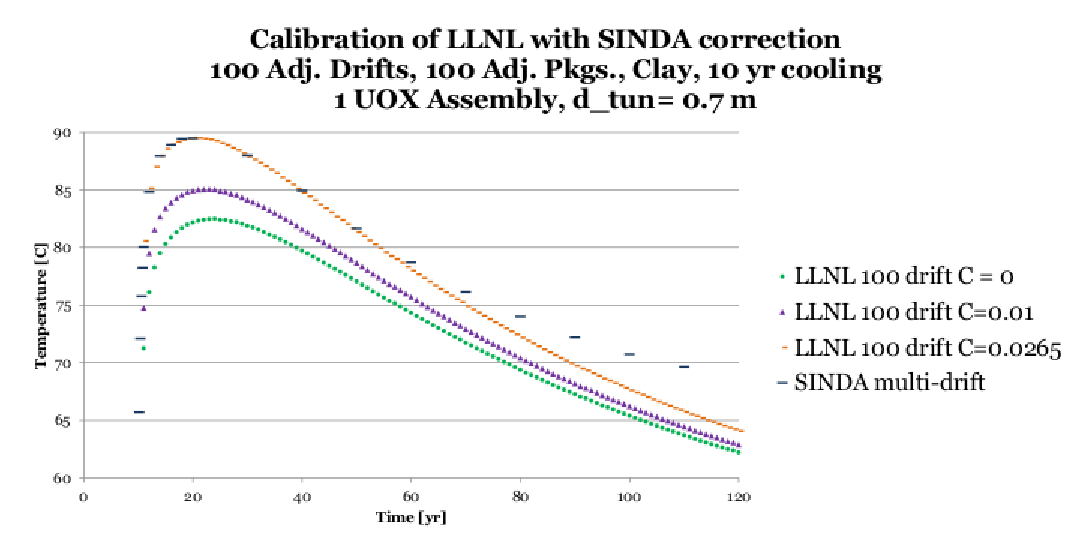
\includegraphics[width=.8\textwidth]{100drift10yr.eps}
      \caption{A multiple drift scenario approximated the inifinite repository 
      scenario run with the SINDA technique.}
    \end{center}
    \label{fig:100drift10yr}
  \end{figure}
\end{frame}

\begin{frame}[ctb!]
  \frametitle{100 Drift 25 year}
  \begin{figure}[h]
    \begin{center}
      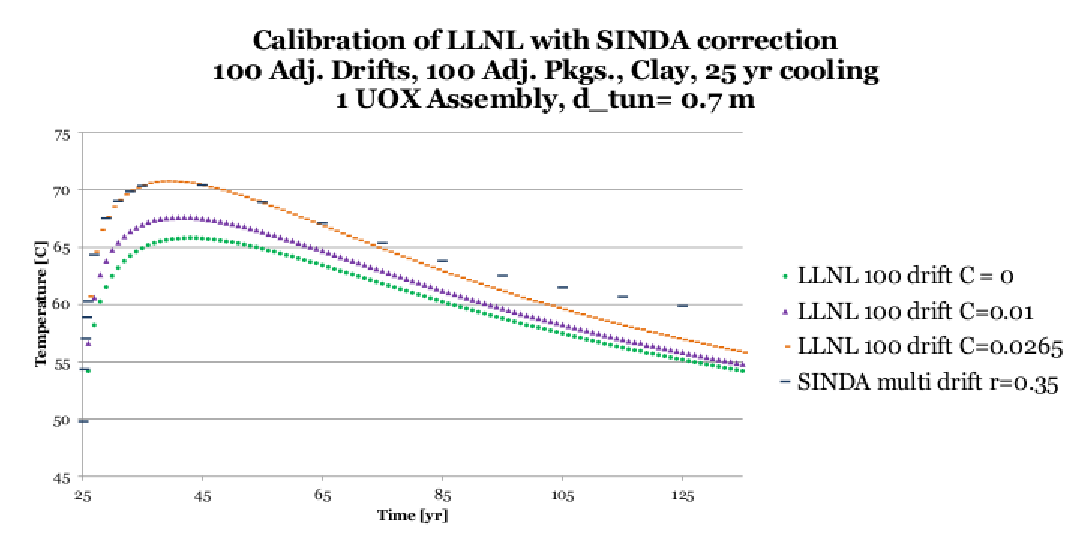
\includegraphics[width=.8\textwidth]{100drift25yr.eps}
      \caption{A multiple drift scenario approximated the inifinite repository 
      scenario run with the SINDA technique.}
    \end{center}
    \label{fig:100drift25yr}
  \end{figure}
  
\end{frame}
\begin{frame}[ctb!]

  \frametitle{100 Drift 50 year}
  \begin{figure}[h]
    \begin{center}
      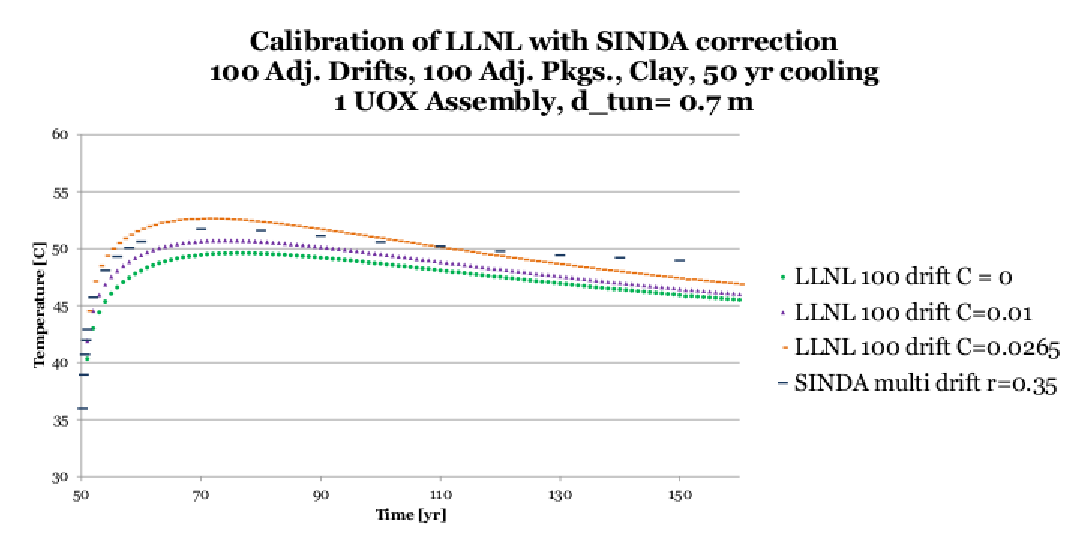
\includegraphics[width=.8\textwidth]{100drift50yr.eps}
      \caption{A multiple drift scenario approximated the inifinite repository 
      scenario run with the SINDA technique.}
    \end{center}
    \label{fig:100drift50yr}
  \end{figure}
  
\end{frame}


\subsection{Single Drift Scenario}

\begin{frame}[ctb!]

  \frametitle{1 Drift 10 year}
  \begin{figure}[h!]
    \begin{center}
      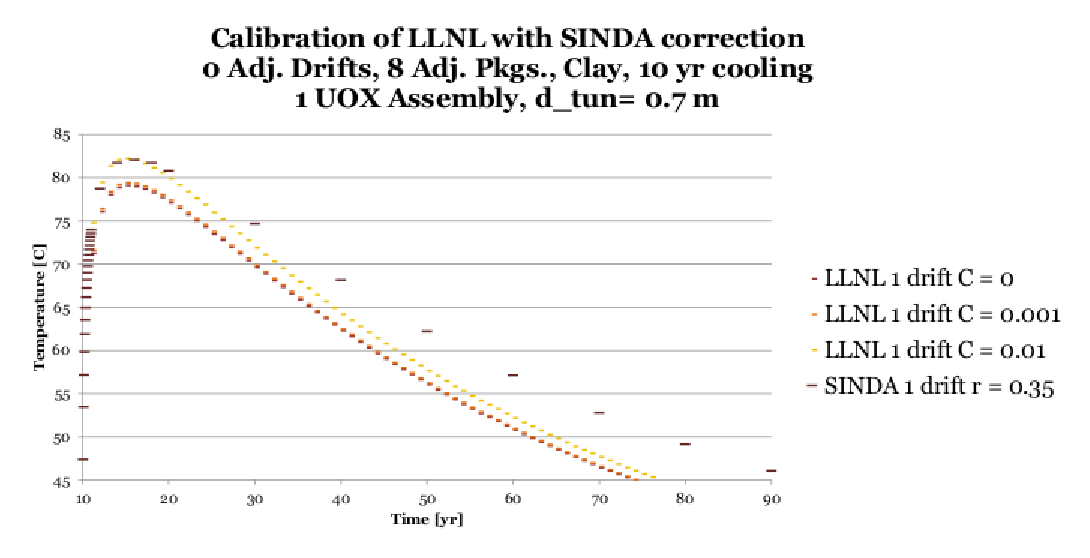
\includegraphics[width=0.8\textwidth]{1drift10yr.eps}
    \end{center}
    \caption{A single drift scenario was compared to the single drift repository 
    scenario run with the SINDA technique.}
    \label{fig:1drift10yr}
  \end{figure}
  
\end{frame}

\begin{frame}[ctb!]

  \frametitle{1 Drift 25 year}
  \begin{figure}[h!]
    \begin{center}
      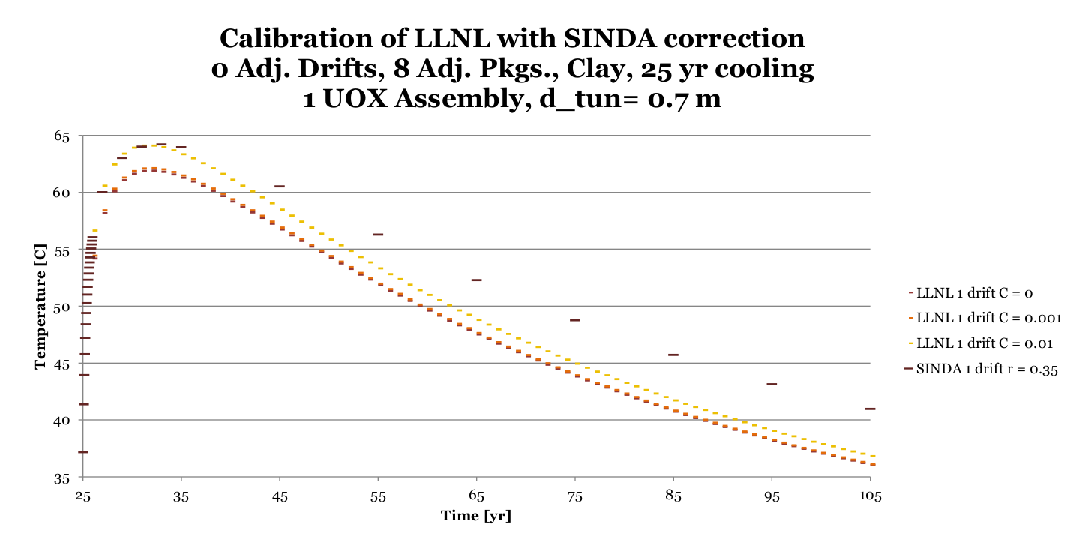
\includegraphics[width=0.8\textwidth]{1drift25yr.eps}
    \end{center}
    \caption{A single drift scenario was compared to the single drift repository 
    scenario run with the SINDA technique.}
    \label{fig:1drift10yr}
  \end{figure}
  
\end{frame}

\begin{frame}[ctb!]

  \frametitle{1 Drift 10 year}
  \begin{figure}[h!]
    \begin{center}
      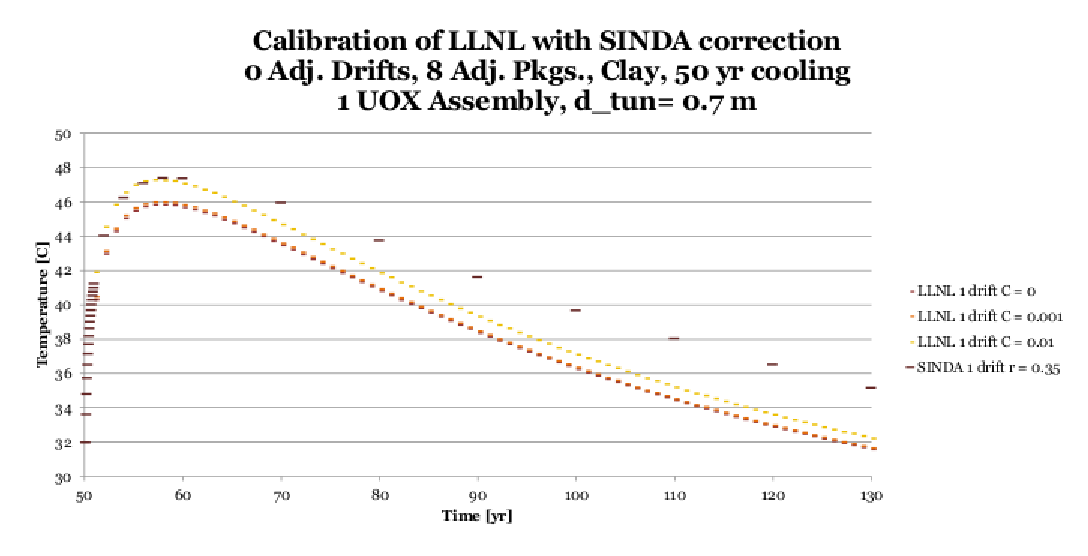
\includegraphics[width=0.8\textwidth]{1drift50yr.eps}
    \end{center}
    \caption{A single drift scenario was compared to the single drift repository 
    scenario run with the SINDA technique.}
    \label{fig:1drift50yr}
  \end{figure}
  
\end{frame}


\subsection{Results and Conclusions}


\begin{frame}[ctb!]
  \frametitle{Summary}
  Benchmarking and calibration of an analytical thermal model against a detailed 
  numerical model showd that the analytical model was accurate within an 
  acceptable range and that it can be adjusted simply. 
\end{frame}



\begin{frame}[ctb!]
  \frametitle{Acknowledgements}  
  This work is supported by the U.S. Department of Energy, Basic Energy 
  Sciences, Office of Nuclear Energy, under contract \# DE-AC02-06CH11357.
\end{frame}




%%--------------------------------%%
%%--------------------------------%%
\begin{frame}[allowframebreaks]
  \frametitle{References}
  \bibliographystyle{plain}
  {\footnotesize \bibliography{ans2012pres} }

\end{frame}

%%--------------------------------%%





\end{document}




